\documentclass[10pt]{article}
\usepackage{graphicx}

\title{Enhancement to eXpOS Operating System and eXpFS File System}

\author{ Kruthika Suresh Ved     B110300CS\\  Sikha V Manoj     B110572CS\\  Sonia V Mathew    B110495CS\\ Guided by: Dr.K.Muralikrishnan}

\usepackage{epsfig}
\begin{document}
	
\maketitle
	

\abstract{} 
Project eXpOS or experimental Operating System is a educational platform to develop an operating system. It is an instructional tool for students to learn and implement OS data structures and functionalities on a simulated machine called XSM (eXperimental String Machine).The OS is programmed using a custom language known as SPL (System Programmer's Language) and application programs, which run on the OS, are programmed using eXpL (Application Programmer's Language).


\section{Problem Definition}
This project aims to modify and update the eXpOS operating system by
\begin{itemize}
\item Re-engineering the eXpFS system. 
\item Including inter process communication
\item Redesigning process model 
\item Introducing shared memory model 
\item Adding more system calls thus broadening the features
\end {itemize}
Thus, adding the above features, eXpOS would become more advanced and closer to operating systems that are available in the market.
\section{eXpOS Specification}
eXpOS has a very simple specification that allows a junior undergraduate computer science student to implement it in a few months, subject to availability of adequate hardware and programming platform support. This OS specification is prepared in a manner independent of programming language and target machine.
\subsection{eXperimental File System (eXpFS)}
eXpOS uses eXpFS (eXperimental File System) which contains files organized into a single directory called the root. There are three types of eXpFS files: the root, data files and executable files. The root is also treated conceptually as a file.
\subsubsection{Root}
The root file has name \textbf {root} and contains information about the files stored in the file system. For each file stored in eXpFS, the root stores three words of information: file-name, file-size and file-type. This triple is called the root entry for the file. The first root entry is for the root itself.  
\subsubsection{Data File}
A data file is a sequence of words. eXpFS expects the Operating System to display data files with an extension .dat.   eXpFS treats this as a default file type, hence the application programs do not have to specify the extension .dat at the time of file creation.  
The operations allowed in data files are Create, Delete, Open, Close, Lock, Unlock, Read, Write, Seek.
\subsubsection{Executable File}
Executable files are essentially program files that must be loaded and run by the operating system.The executable file format recognized by eXpOS is called the Experimental executable file (XEXE) format. In this format, an executable file is divided into three sections - Header and Code. In this implementation of eXpOS, static data is stored in stack pages.
\subsection{Process Model}
A program under execution is called a process. The eXpOS associates a virtual (memory) address space for each process. The eXpOS logically partitions the address space into four regions: library, code, stack and heap. These regions are mapped into physical memory using hardware mechanisms like paging/segmentation.
%\begin{figure}[ht]
%\centering
%\includegraphics[scale=0.75]{P_Model.png}
%\caption{\footnotesize Process Model in eXpOS}
%\label{fig_1}
%\end{figure}
\subsection{Inter-Process Communication}
eXpOS assumes a single processor multi programming environment. It allows processes to communicate with each other using mechanisms like semaphores and Wait-Signal system calls.
eXpOS provides (binary) semaphores to allow application programs to handle the critical section problem. eXpOS provides system calls like Semget, SemLock, SemUnlock, Semrelease for working with semaphores.
\subsection{Shared Memory Model}
Shared memory is an efficient means of sharing data between programs. In eXpOS, this sharing is done between the parent process and child processes through heap. It is the responsibility of the programmer to ensure exclusive access to the shared resources for each process, to avoid data inconsistency. eXpOS helps programmer to realize data consistency with the help of semaphores. 
\subsection{System Calls}
When a process invokes a system call, the process is interrupted and control goes to the kernel. Once the system call is carried out, the control goes back to user mode. There are system calls associated with processes, files and semaphores.\\
The following system calls are present in the system: 
\begin{itemize}
\item File System Calls : Create, Delete, Open, Close, Read, Write, Seek
\item Process System Calls : Fork, Exec, Exit, Getpid, Getppid, Shutdown
\item System calls for access control and Synchronization: Wait, Signal, FLock, FUnLock, Semget, Semrelease, SemLock, SemUnLock.
\end{itemize}

\subsection{Pre-Emptive Scheduling}
In Pre-Emptive Scheduling, process can be paused before its time slice is over. This usually happens when a resource that the process requires is not available at the present. It puts itself to sleep and another process can be scheduled for execution.
\subsection{Asynchronous disk operations}
To minimize processor cycles spent on disk operations, disk operations were made asynchronous. This means that while a disk operation is being carried out, other processes which do not require the disk can be executed.
\section{Design of eXpOS}
\subsection{Data Structures}
It can be divided into - Disk Data structures and Memory (in-core) data structures. A copy of Disk Data Structures will be kept in the memory while the system is on, for reducing disk access.
\subsection{Disk Data Structures}
\subsubsection{Inode Table}
Inode Table is the record of the files stored in the disk. The entry of an Inode table has the following format:
\begin{figure}[ht]
\centering
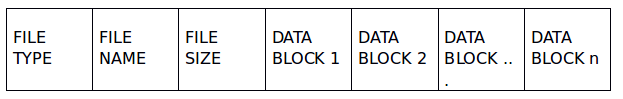
\includegraphics[scale=0.50]{Inode_table.png}
\caption{\footnotesize Structure of the Inode Table}
\label{fig_1}
\end{figure}
\subsubsection{Disk Free List}
For each block in the disk there is an entry in the Disk Free List which contains a value of either 0 or 1 indicating whether the corresponding block in the disk is free or used, respectively.
\subsection{Memory Data Structures}
\subsubsection{Process Table}
 The Process Table contains an entry for each process.  Each entry contains several fields that stores all the information pertaining to a single process and the maximum number of entries is equal to maximum number of processes allowed to exist at a single point of time in eXpOS.
\begin{figure}[ht]
\centering
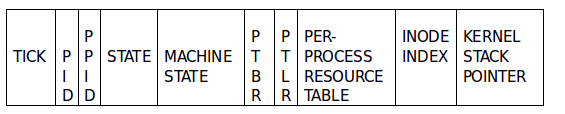
\includegraphics[scale=0.50]{Process_table.png}
\caption{\footnotesize Structure of the Process Table}
\label{fig_1}
\end{figure}

The first entry Tick keeps track of how long the process was in memory. \\
The second column is PID or Process ID which is the unique process descriptor, a number that is unique to each process.\\ 
The third column gives the process descriptor of the parent process or the PPID.\\
Next column, State , consists of a two tuple that describes the current state of the process.\\
The fifth column is the pointer to a structure that gives the Machine State when the process was last executed.  This part is machine dependent. \\
The next two columns are regarding page table of the process. The first one (PTBR or Page Table Base Register) stores the starting address of the page table of a process while the next one (PTLR or Page Table Length Register) stores the number of entries in the page table of a process and determines the size of the virtual address space of the process.\\
The next column is a pointer to a table, the Per-Process Resource Table that contains information about the files opened by the process as well as semaphores used by the process.The index of the per-process resource table entry for each resource is known as the resource descriptor.\\
Inode Index is a reference to the Inode entry of the executable file. It could be used to access the code pages of the process.\\
Each process has its own kernel stack whose pointer is given in the Kernel Stack Pointer column. A process uses its kernel stack to save the return address when it decides to voluntarily schedule out itself out when entering a blocking system call. 
\subsubsection{File Table}
File Table has information about all the files that are currently open.  It is initialized by the OS startup code.  Initially, there are no open files.
\begin{figure}[ht]
\centering
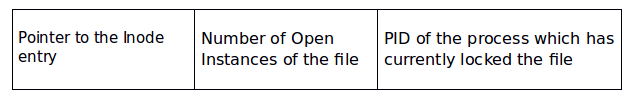
\includegraphics[scale=0.50]{File_table.png}
\caption{\footnotesize Structure of the File Table}
\label{fig_1}
\end{figure}
\subsubsection{Semaphore Table}
Semaphore Table contains details about all the semaphores used by the processes. For every semaphore opened by a process, there is an entry in the per-process resource table (which is discussed later),  and this entry points to a corresponding entry in the semaphore table.
\begin{figure}[ht]
\centering
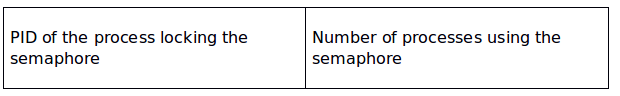
\includegraphics[scale=0.50]{Semaphore_Table.png}
\caption{\footnotesize Structure of the Semaphore Table}
\label{fig_1}
\end{figure}
\subsubsection{Disk Status Table}
eXpOS makes use of Disk Status Table to keep track of load and store operations. It consists of four entries which is given in Figure 4.
\begin{figure}[ht]
\centering
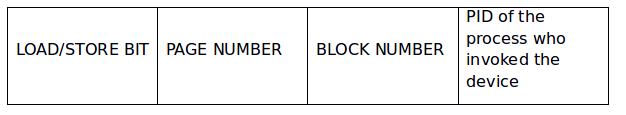
\includegraphics[scale=0.50]{Disk_Status.png}
\caption{\footnotesize Structure of the Disk Status Table}
\label{fig_1}
\end{figure}
\\ \\
\subsubsection{Buffer Table}
To minimize the number of load and store operations, eXpOS provides a buffer cache in memory which would temporarily store disk blocks. Each disk block is mapped to a unique buffer. The disk blocks will be stored back to the disk when some other blocks replace it. Only modified blocks are written back to disk.
Buffer Table keeps the information about disk blocks present in the buffer.
\begin{figure}[ht]
\centering
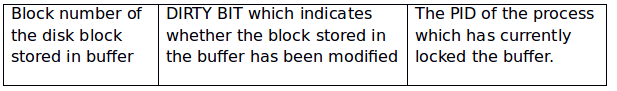
\includegraphics[scale=0.50]{Buffer_table.png}
\caption{\footnotesize Structure of the Buffer Table}
\label{fig_1}
\end{figure}
\subsubsection{System Status Table}
System Status Table keeps the information about number of free pages in memory (Mem\_free\_count), number of processes waiting for memory pages (Wait\_mem\_count) , and also the number of processes in swapped state (Swapped\_count).
\subsubsection{Memory Free List}
The Memory free list is a data structure used for keeping track of used and unused pages in the memory. Each entry of the free list contains a value of either 0 indicating whether the corresponding page in the memory is free or number indicating the number of processes that share the page.
\subsection{Algorithms}
\subsubsection{File System Calls}
\textbf{Create System Call}\\
The Create operation takes as input a filename and creates an empty file by that name. It also creates the root entry for the file and makes sure that every file has a unique name. Note that the file name must be a character string and must not be named “root”.
\begin{description}
\item[Arguments]: Filename
\item[Return Value]: 0 (Success) or -1 (No Space for file)
\end{description} 
\begin{enumerate}
\item Inode Table Validation  \\
The memory copy of Inode table is searched for Filename. If the entry is found, return from the system call with 0, indicating success. If not, check for free entry in Inode Table. If there is no free entry, return from system call with error code -1. If an entry is found, store the index in InodeIndex.
\item Updating Inode Table\\
In the entry corresponding to InodeIndex, set the file name field with Filename. The File size field is initialized to 0. Set the file type field as “DATA ”.
\item Update the root file entry
The entry for the file in the root is at InodeIndex. Set the filename field with Filename, file size to 0 and file type as “DATA”.
\item Return from the system call with return value 0, indicating success.
\end{enumerate}
\section{Work Done}
\begin {itemize}
\item The existing OS data structures were redesigned to incorporate the changes done. 
\item New data structures like Buffer Table, Disk Status Table, Semaphore Table etc were designed.
\item System calls were redesigned to incorporate asynchronous operations, buffer cache and pre-emptive scheduling.
\item Directory structure was introduced in eXpFS.
\item Executable file format was designed.
\end{itemize}
 
\section{Future Work}
Future work includes implementation of all the features mentioned above, testing of the system and building a roadmap for anyone wishing to build eXpOS.
\section{Conclusion}
This project aims to create a simpler version of an operating system which allows students to acquire insight into the working of a real operating system. 

\begin{thebibliography}{1}
\bibitem{latexMath}\texttt{$http://xosnitc.github.io/$}
\bibitem {2} The Design of Unix Operating System, By Maurice J. Bach
\end{thebibliography}

\end{document}
